 %To Ajit: Please use the built in commenting functionality in overleaf, this helps me structure things, also, if there is any grammar errors or similar that you would like to correct, please have "track changes" switched on so i can see what you change. Thank you.

\chapter{Method}\label{chap:Method}
This chapter starts of with presenting issue with the lidar's blind-zone, and illustrates this with several figures. The experimental setup is presented next, where the major hardware are discussed in detail, like the ranging sensors and the mounting system for the radar modules. An overview of the system initialisation are presented in the algorithm section. The ROS system is explained lastly, including the ROS1 perception system, ROS2 navigation and robot control and the ROS1 bridge.

The resources for this project exists a GitHub repository. The repository consists of several branches, where the main branch is dedicated to this document and documentation pursues. The other branches mainly contain ROS files for different stages of the project. The "nav" branch is the latest and most up to date branch, and it is the branch that should be considered when trying to re-create this project. Link to GitHub reposetory: \url{https://github.com/didriknr/Master-thesis-Didrik-Robsrud}

\section{Problem to solve}% this part fits well in the experimental setup section.
The Husky was equipped with a 3D-lidar before this project started, which have been used for autonomous navigation in a previous project \cite{uia_husky_0776}. While the lidar can detect objects at a distance of $120 m$, is cannot determine the distance to objects closer than $0.8m$. This combined some other factors, which will be discussed in \ref{subsec:Lidar}, results in a problematic blind zone for the system. Figure \ref{fig:lidarFovLeftSketchLimited} and \ref{fig:lidarFovTopSketch} illustrates the FOV of the lidar\footnote{Note that all the figures in this chapter illustrating FOV are not properly scaled and deviates somewhat from reality. The FOV of the lidar appears to be better than it really is.}, seen from the side and the top, respectively. The bottom line in figure \ref{fig:lidarFovLeftSketchLimited} represents the ground, and its ends represents where the lidar FOV would have intercepted the ground if it wasn't for the configuration done in \ref{subsubsec:lidar.launch}. The other lines represents the FOV of the lidar, which is capped at $\pm 1 m$ relative to the lidar. Everything outside of these lines are part of the systems blind zone. Objects outside the systems FOV cannot be detected. 

\begin{figure}[H]
    \centering
    \begin{minipage}[b]{0.49\textwidth}
        \includegraphics[width=\textwidth]{Figures/CAD/FOV/lidarFovLeftSketchLimited.PNG}
        \caption{Left view of the lidar's field of view. The horizontal line underneath the Husky represents the ground. The triangle like shape surrounding the husky represents the blind zone. The other lines represents the borders of the FOV of the lidar.}
        \label{fig:lidarFovLeftSketchLimited}
    \end{minipage}
    %\hfill
    \begin{minipage}[b]{0.49\textwidth}
        \includegraphics[width=\textwidth]{Figures/CAD/FOV/lidarFovTopSketch.PNG}
        \caption{Top view of the lidar's field of view. The circle surrounding the Husky represents the blind zone of the lidar, it can see outeside of it up to $120 m$.}
        \label{fig:lidarFovTopSketch}
    \end{minipage}
\end{figure}
%aj a lot of white space between figure and caption. remove white space.
The aim of this project is to remedy the poor blind-zone of the lidar with the help of two radar modules. This should result in safer indoor navigation, with better collision avoidance. Figure \ref{fig:lidarAndRadarFovLeftSketchMergedLimited} and \ref{fig:lidarAndRadarFovTopSketchMerged} illustrates the FOV of the lidar and the radars combined, seen from the side and the top, respectively. The figures illustrates a clear improvement in the system's combined FOV. See section \ref{subsec:Radar} for more information.

\begin{figure}[H]
    \centering
    \begin{minipage}[b]{0.49\textwidth}
        \includegraphics[width=\textwidth]{Figures/CAD/FOV/lidarAndRadarFovLeftSketchMergedLimited.PNG}
        \caption{Left view of the lidar's and radars' combined field of view. Similar to figure \ref{fig:lidarFovLeftSketchLimited}, but with the addition of the radars' FOV improving the system's combined FOV.}
        \label{fig:lidarAndRadarFovLeftSketchMergedLimited}
    \end{minipage}
    %\hfill
    \begin{minipage}[b]{0.49\textwidth}
        \includegraphics[width=\textwidth]{Figures/CAD/FOV/lidarAndRadarFovTopSketchMerged.PNG}
        \caption{Top view of the lidar's and radars' combined field of view. Similar to figure \ref{fig:lidarFovTopSketch}, but with the addition of the radars' FOV improving the system's combined FOV.}
        \label{fig:lidarAndRadarFovTopSketchMerged}
    \end{minipage}
\end{figure}

Figure \ref{fig:lidarAndRadarFovLeftSketch} and \ref{fig:lidarAndRadarFovTopSketch} are similar to figure \ref{fig:lidarAndRadarFovLeftSketchMergedLimited} and \ref{fig:lidarAndRadarFovTopSketchMerged}, but with where the lines that represent the borders of the FOV for the lidar and radars are uninterrupted (within the picture frame). This makes it easier to see the contribution to the FOV of each of the sensors. 

\begin{figure}[H]
    \centering
    \begin{minipage}[b]{0.49\textwidth}
        \includegraphics[width=\textwidth]{Figures/CAD/FOV/lidarAndRadarFovLeftSketch.PNG}
        \caption{Left view of the lidar's and radars' overlapping field of view. This figure is similar to figure \ref{fig:lidarAndRadarFovLeftSketchMergedLimited}.}
        \label{fig:lidarAndRadarFovLeftSketch}
    \end{minipage}
    %\hfill
    \begin{minipage}[b]{0.49\textwidth}
        \includegraphics[width=\textwidth]{Figures/CAD/FOV/lidarAndRadarFovTopSketch.PNG}
        \caption{Top view of the lidar's and radars' overlapping field of view. This figure is similar to figure \ref{fig:lidarAndRadarFovTopSketchMerged}.}
        \label{fig:lidarAndRadarFovTopSketch}
    \end{minipage}
\end{figure}

\section{Experimental setup} % experiment setup - content of 2.1 and 2.1.1 goes here
This section will go trough the the hardware and software setup of this project. Figure \ref{fig:HWdiagram} presents the most important hardware used in the system and how it communicates. The lidar, Radar0 and Radar1 are all range sensors used for autonomous navigation, see sections \ref{subsec:Lidar} and \ref{subsec:Radar} for more information. The Husky is the robot-platform used in this project, see section \ref{subsec:Husky} for more information. The operator computer is a laptop running Ubuntu which is used to interface with the system trough ROS and SSH. The Joy-stick, called "F710 Wireless Gamepad"\cite{logitechF710}, is used to drive the Husky manually. The IMU used is called UM7 \cite{redshiftlabs-um7}. The single board computer (SBC) used as the UGV's onboard computer is called Jetson AGX Xavier \cite{jetson-agx-xavier-user-guide}.

\begin{figure}[H]
    \centering
    \includegraphics[scale=1]{Figures/draw.io/hardwareBlockDiagram.drawio.pdf}
    \caption{Hardware diagram of system}
    \label{fig:HWdiagram}
\end{figure}
Figure \ref{fig:huskyWithSensors} displays a CAD model of the system which shows how the most important hardware is mounted. Figure \ref{fig:testSetupClose} shows a image of the system.
% aj lot of white space between figure and caption ?
\begin{figure}[H]
    \centering
    \begin{minipage}[b]{0.49\textwidth}
        \includegraphics[width=\textwidth,trim={ 7.5cm 2.5cm 7.5cm 5cm},clip]{Figures/CAD/huskyWithSensors.PNG}
        \caption{CAD model of system.}
        \label{fig:huskyWithSensors}
    \end{minipage}
    %\hfill
    \begin{minipage}[b]{0.49\textwidth}
        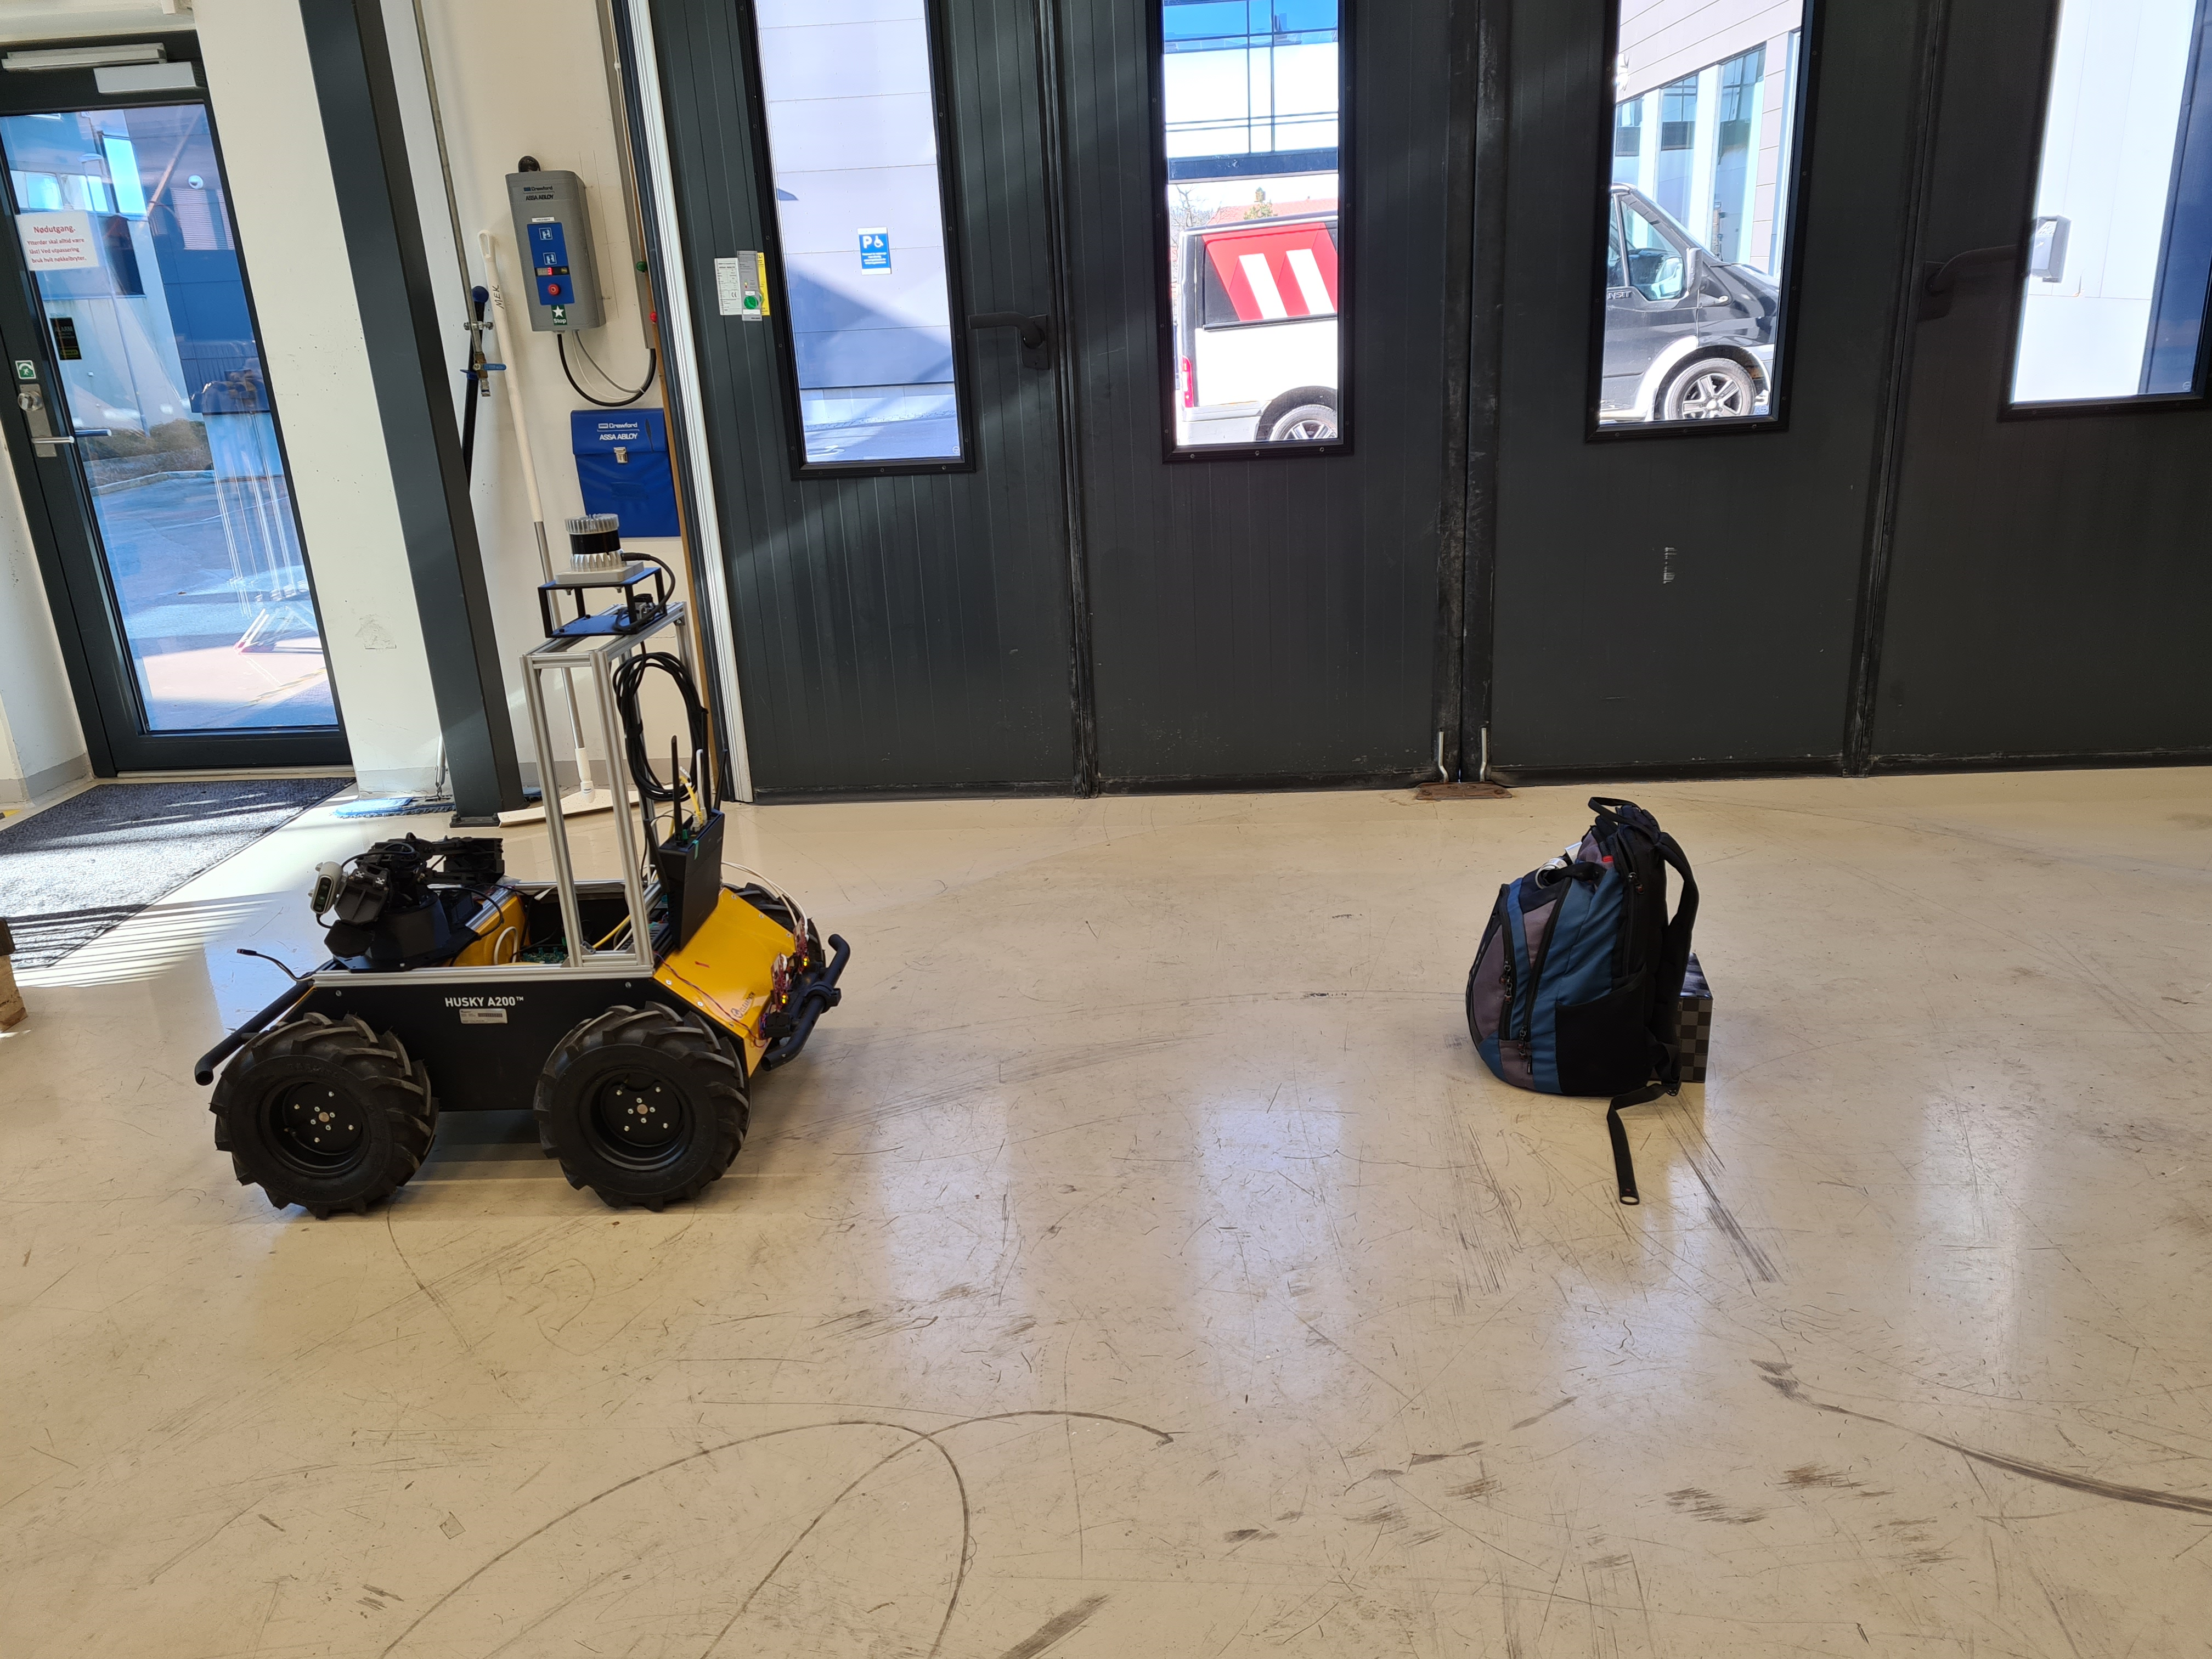
\includegraphics[width=\textwidth,trim={ 12cm 28cm 87cm 32.5cm},clip]{Figures/testSetup.png}
        \caption{Picture of system. Zoomed in version of figure \ref{fig:testSetup}.}
        \label{fig:testSetupClose}
    \end{minipage}
\end{figure}

%\subsection{Sensors}
\subsection{Lidar}\label{subsec:Lidar}
The lidar used in this project is called OS1 and is a product by Ouster. The lidar has got a minimum range of $0.8 m$ and a maximum of $120 m$. The has a vertical FOV of $\pm 16.6 ^\circ$, and a horizontal FOV of $360 ^\circ$ \cite{ousterOS1datasheet}. The lidar is mounted such that the centre of the "glass-part" (the black part) sits approximately $1026 mm$ above the ground. 

Figure \ref{fig:lidar} displays a CAD model of the lidar, obtained from \cite{ouster-download}. This is also the source for the aluminium mount that sits directly below the lidar in figure \ref{fig:lidarMounted}. The box-like structure sitting below the aluminium lidar mount was created by \cite{muggerud2023} and \cite{ovsthus2023}. The aluminium frame that makes up the tower that holds up the lidar was made by \cite{ovsthus2023}. 

\begin{figure}[H]
    \centering
    \begin{minipage}[b]{0.49\textwidth}
        \includegraphics[width=\textwidth]{Figures/CAD/lidar.PNG}
        \caption{CAD model of the lidar.}
        \label{fig:lidar}
    \end{minipage}
    %\hfill
    \begin{minipage}[b]{0.49\textwidth}
        \includegraphics[width=\textwidth]{Figures/CAD/lidarMounted.PNG}
        \caption{lidar mounted to the rest of the system.}
        \label{fig:lidarMounted}
    \end{minipage}
\end{figure}

\subsection{Radar}\label{subsec:Radar}
The radar modules used in this project are produced by Texas instruments as an evaluation evaluation board for the AWR1843 radar chip \cite{awr1843boost}. The evaluation board is called AWR1843BOOST. The FOV for both of the radar modules intersects the ground at an angle of $14 ^{\circ}$ approximately $1336 mm$ in front of the radar modules (assuming values from \cite{xWR1843EvalModule}). The antenna centre of both of the
radar modules are positioned at about 333mm above the ground.

Figure \ref{fig:radar} shows a 3D-CAD (Computer Aided Drawing) of the radar module, which was obtained form \cite{awr1843boost3dmodel}. This CAD model has been used in the design of the radar mounting system, in the creation of a URDF file for the radar module, and as a visualisation tool. The Solidworks URDF exporter tool \cite{sw_urdf_exporter} was used to create the URDF file of the radar. A video guide was used to understand the tool \cite{solidworksURDFExport}. The URDF file was created to ensure that the reference frames of the radar would get properly positioned relative to the rest of the ROS system, like the centre of the antenna. Also, a URDF file did not already exist in the ROS package for the radar. Two links, or reference frames was created for the URDF file. One of the frames are positioned in the middle of the mounting-holes near the bottom of the PCB (Printed Circuit Board) of the module, and second frame is positioned in the middle of the antenna patch, at the outer surface. 

\begin{figure}[H]
    \centering
    \begin{minipage}[b]{0.49\textwidth}
        \includegraphics[width=\textwidth]{Figures/CAD/radar.PNG}
        \caption{CAD model of radar module.}
        \label{fig:radar}
    \end{minipage}
    %\hfill
    \begin{minipage}[b]{0.49\textwidth}
        \includegraphics[width=\textwidth]{Figures/CAD/radarMounted.PNG}
        \caption{Close up view of one of the radar modules mounted to the rest of the system.}
        \label{fig:radarMounted}
    \end{minipage}
\end{figure}

Finding the position of the antenna centre was challenging, as no written documentation on this was found. The position of the antenna patch was obtained by inserting a picture of the radar (seen in figure \ref{fig:AWR1843BOOST_DSL}) on top of the CAD model. This was done similarly to a video guide \cite{reverseEngineeringSOLIDWORKS}. A rectangle was drawn around the RX-part of the antenna patch (\cite{xWR1843EvalModule}), and then extruded to create a box. A point can then be created at the centre of the box, at the surface facing the "screen" in figure \ref{fig:radarAntenna}. This point can then be projected on to the surface of the PCB to produce a point representing the centre of the RX part of the antenna patch. The box also serves as a dummy-object in the URDF-process, because (seemingly) each frame requires a body/object to be associated with it. The dummy-object was removed after the URDF was generated, by editing the URDF file, and deleting the \textit{stl} file of the box that was generated to go along with the URDF file. 


\begin{figure}[H]
    \centering
    \begin{minipage}[b]{0.49\textwidth}
        \includegraphics[width=\textwidth]{Figures/AWR1843BOOST_DSL.png}
        \caption{Front view picture of the AWR1843BOOST radar module \cite{awr1843boostImage}}
        \label{fig:AWR1843BOOST_DSL}
    \end{minipage}
    %\hfill
    \begin{minipage}[b]{0.49\textwidth}
        \includegraphics[width=\textwidth]{Figures/CAD/radarAntenna.PNG}
        \caption{Front view of CAD model of radar, with a grey box representing the left part of the antenna patch}
        \label{fig:radarAntenna}
    \end{minipage}
\end{figure}

A online tool was used in the beginning of the project to interface with the radar modules. This tool allowed some settings to be altered and the ranging data to be visualised in real time plots. See \cite{mmwaveVisualizerWebsite} to access the tool.

\subsection{Mounting system}

% use paragraph for each item for mounting \paragraph{}
Each of the radar modules was packaged with metal legs with rubber-like feet, and screws and nuts to fasten them to the PCB. This setup was used in early stages of the project with the radar modules standing on a desk. The radar modules was later placed on top of the front bumper/rail of the Husky. They were fastened by tangling the legs underneath the excessive cable of the lidar. This poor setup can be seen in figure \ref{fig:badRadarMount}, where a roll of red electrician tape was used to prop up the modules. There are several reasons why this is a poor solution, but one is that it is difficult to determine the position of the modules, which becomes important when the ranging data from the radars are going to be used in ROS. 

\begin{figure}[H]
    \centering
    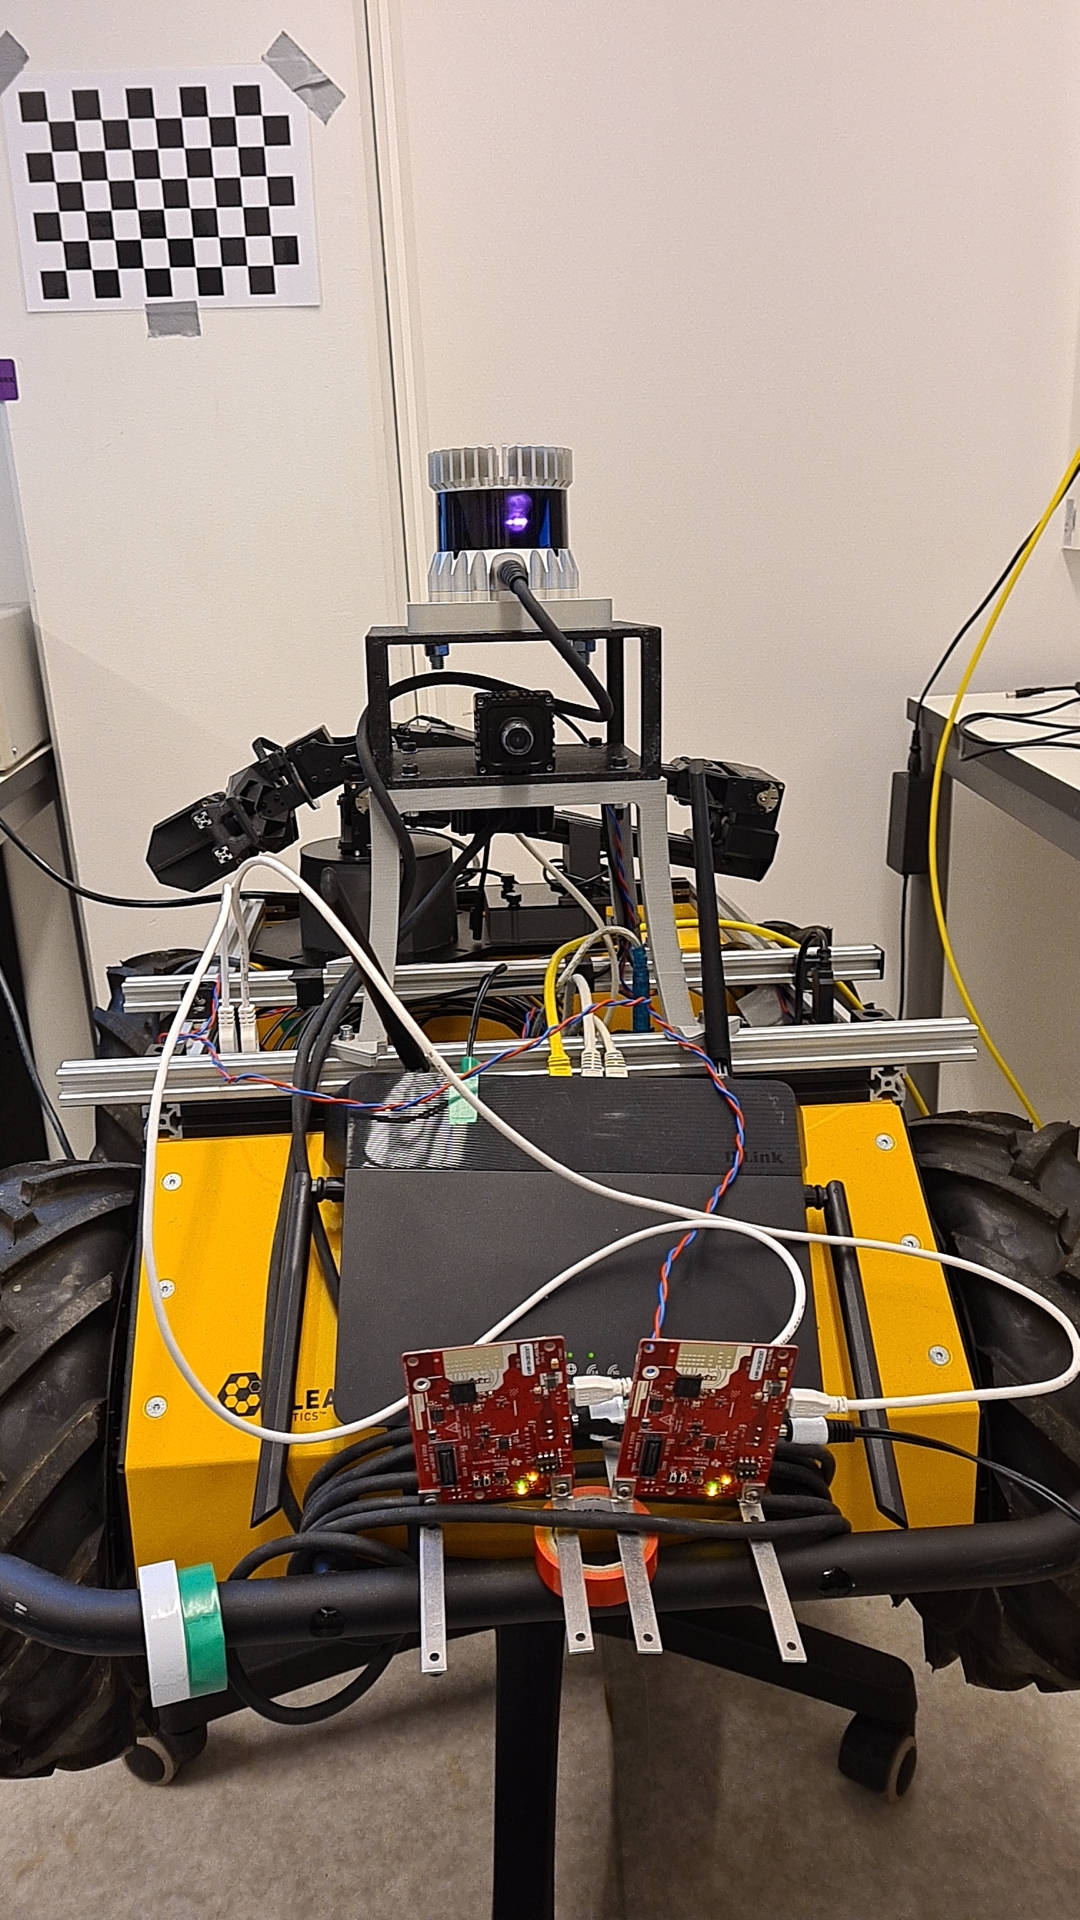
\includegraphics[scale=0.4,trim={ 0 2.5cm 0 10cm},clip]{Figures/badRadarMount.png}
    \caption{Sub optimal mounting of radar modules. Picture was taken early in the project.}
    \label{fig:badRadarMount}
\end{figure}

A mounting system was created to securely mount the radar modules to the front bumper of the Husky. The bumper was chosen as a mounting location as it is in front of the vehicle and relatively near the ground. The mounting system has got two crucial requirements to meet: it should attach to the bumper bumper in a predictable way, with little to no wiggle room, so it is easy to determine its position, and it has to be able to hold the radar modules in a similarly predictable way. Figure \ref{fig:upperRadarMountV2} illustrates the radar mount part of the system, figure \ref{fig:radarmountMounted} displays the radar mount assembled together with the rest of the system. The mounting system was realised trough FDM 3D printing. The parts was printed in PLA. The following chapters will explain the considerations made when the mounting system was created. 

\begin{figure}[H]
    \centering
    \begin{minipage}[b]{0.49\textwidth}
        \includegraphics[width=\textwidth]{Figures/CAD/upperRadarMountV2.PNG}
        \caption{CAD model of the radar mount.}
        \label{fig:upperRadarMountV2}
    \end{minipage}
    %\hfill
    \begin{minipage}[b]{0.49\textwidth}
        \includegraphics[width=\textwidth]{Figures/CAD/radarmountMounted.PNG}
        \caption{The radar mount mounted to the rest of the system.}
        \label{fig:radarmountMounted}
    \end{minipage}
\end{figure}
%\subsubsection{Mounting to the bumper}
\paragraph{Mounting to the bumper.}
The Husky boast one front - and one back bumper, which appear to be equal. The mounting system should work on both bumpers, but has only been tested and designed for the front bumper. A generic mount has been designed as a template for creating different mounts, but also as a support for the radar mount as seen in figure \ref{fig:radarmountMounted}. Figure \ref{fig:GenericMountV2} displays the generic mount. The Generic mount consist of three clamping structures and a flat area connecting them. The two smaller clamping structures are meant to hold up the mounting system and preventing it from altering its pitch (angle). The third, bigger clamping structure is mainly meant to prevent the rest of the mounting system to slide back and forth on the two parallel rods attaching the bumper to the rest of the Husky. The bigger clamping structure are likely improving wiggling in the yaw-direction of the mounting system as well. The clamping structures have two holes meant for the screws and nuts that are included with the radar modules, which are of the M3-type \cite{awr1843boostintro}. The holes are sunk and has a chamfer at the top. Such holes are also present near the middle of the mount. The clamping structures also has a channel that allows a cable tie to be used to fasten the mounting system. Thus the mounting system can be fastened by screws and nuts or cable ties, or both. Figure \ref{fig:upperRadarMountV2CloseUp1} displays a clamping structure of the radar mount, which possesses the same holes and channels as the generic mount.

\begin{figure}[H]
    \centering
    \begin{minipage}[b]{0.49\textwidth}
        \includegraphics[width=\textwidth]{Figures/CAD/GenericMountV2.PNG}
        \caption{Generic mount.}
        \label{fig:GenericMountV2}
    \end{minipage}
    %\hfill
    \begin{minipage}[b]{0.49\textwidth}
        \includegraphics[width=\textwidth]{Figures/CAD/upperRadarMountV2CloseUp1.PNG}
        \caption{Close up view of a clamping structure of the radar mount.}
        \label{fig:upperRadarMountV2CloseUp1}
    \end{minipage}
\end{figure}

The mounting system has been designed such that there is a $1 mm$ distance between the top and bottom part, as seen in figure \ref{fig:mount0radar}. The inner radius of the clamping structures are also slightly greater than the outer radius of their corresponding rods.

\begin{figure}[H]
    \centering
    \includegraphics[scale=0.5]{Figures/CAD/mount0radar.PNG}
    \caption{Mounting system}
    \label{fig:mount0radar}
\end{figure}
%\subsubsection{Mounting to the radar modules}
\paragraph{Mounting to the radar modules.}
The radar mount are designed so that a radar module can be mounted at three different locations. This allow for two configurations, a single radar module mounted in the middle, or two radar modules on the sides, as seen in figure \ref{fig:uppermount1radar} and \ref{fig:uppermount2radar}, respectively. Mounting three modules at the radar mount is unfeasible as the power - and data cables will have difficulties fitting. 

\begin{figure}[H]
    \centering
    \begin{minipage}[b]{0.49\textwidth}
        \includegraphics[width=\textwidth]{Figures/CAD/uppermount1radar.PNG}
        \caption{Radar mount with one radar module mounted.}
        \label{fig:uppermount1radar}
    \end{minipage}
    %\hfill
    \begin{minipage}[b]{0.49\textwidth}
        \includegraphics[width=\textwidth]{Figures/CAD/uppermount2radar.PNG}
        \caption{Radar mount with two radar modules mounted.}
        \label{fig:uppermount2radar}
    \end{minipage}
\end{figure}

The radar modules are fastened to the mount trough two pillar like support fixtures. One of these pillars can be seen in figure \ref{fig:upperRadarMountV2CloseUp1}, sitting on top of the clamping structure. Figure \ref{fig:radarMounted} shows how a radar module mounts to the pillars. Figure \ref{fig:upperRadarMountV2TopView} shows a top view of the radar mount, illustrating the six pillars and that they consist of three walls. The side walls of the pillar are shaped so they are as tall as the front wall where they contact it, then they slant toward the surface they sit on, as seen in figure \ref{fig:upperRadarMountV2LeftView}. The walls are spaced so the nuts that where included, with the radar modules, fits loosely between them, but cannot rotate, which makes assembly more convenient. Figure \ref{fig:upperRadarMountV2FrontView} displays the holes in the front wall where the fastening screws, that holds the radar modules, go trough. This figure also illustrates that the two middle pillars are not symmetrically positioned, this is done so the radar module will be centred when it is in this position as the holes at the bottom of the PCB are not symmetrical positioned, this consideration was not made for the other positions. The holes has the same radius as the corresponding holes on the PCB of the radar modules. There is a small ledge on the front wall of the pillars on which the PCB can rest upon, and the edge where the ledge meets the font wall should be the only sharp inner edge of the mounting system (except for the letters). 

\begin{figure}[H]
    \centering
    \begin{minipage}[b]{0.49\textwidth}
        \includegraphics[width=\textwidth]{Figures/CAD/upperRadarMountV2FrontView.PNG}
        \caption{Front view of radar mount.}
        \label{fig:upperRadarMountV2FrontView}
    \end{minipage}
    %\hfill
    \begin{minipage}[b]{0.49\textwidth}
        \includegraphics[width=\textwidth]{Figures/CAD/upperRadarMountV2LeftView.PNG}
        \caption{Left view of radar mount.}
        \label{fig:upperRadarMountV2LeftView}
    \end{minipage}
\end{figure}

\begin{figure}[H]
    \centering
    \includegraphics[scale=0.5]{Figures/CAD/upperRadarMountV2TopView.PNG}
    \caption{Top view of radar mount}
    \label{fig:upperRadarMountV2TopView}
\end{figure}

The radar module has got a pin sticking out on its backside, which prevented the radar modules to be mounted to the first iteration of the radar mount. This pin can be observed near the hole of the PCB in figure \ref{fig:radarBackCloseUpOfPin}. This issue was addressed by creating a indentation in the outer wall on the left side of the pillars interacting with the right hole of the radar PCB. This indentation can be seen in figure \ref{fig:upperRadarMountV2CloseUp2}, which gives a close up view of the right-middle pillar. %The appearance of the indentations can be observed in figure 

\begin{figure}[H]
    \centering
    \begin{minipage}[b]{0.49\textwidth}
        \includegraphics[width=\textwidth]{Figures/CAD/radarBackCloseUpOfPin.PNG}
        \caption{Pin sticking out of the backside of the radar module's PCB.}
        \label{fig:radarBackCloseUpOfPin}
    \end{minipage}
    %\hfill
    \begin{minipage}[b]{0.49\textwidth}
        \includegraphics[width=\textwidth]{Figures/CAD/upperRadarMountV2CloseUp2.PNG}
        \caption{Close up view of the right-middle pillar with a dent complying with the pin in figure \ref{fig:radarBackCloseUpOfPin}.}
        \label{fig:upperRadarMountV2CloseUp2}
    \end{minipage}
\end{figure}

%\begin{figure}[H]
%    \centering
%    \includegraphics[scale=0.5]{Figures/CAD/GenericMountV22.PNG}
%    \caption{Top view of radar mount}
%    \label{fig:upperRadarMountV2TopView}
%\end{figure}

%\subsubsection{URDF}
\paragraph{URDF}
A URDF file was made for the radar mount with the same method as for the radar module (\ref{subsec:Radar}), but with some deviation. The radar mount URDF consists of four reference frames, where one base frame lays on top of the Husky's base frame. The the other frames are placed where the the base frame of the radar modules would be, almost. The frames for the radar positions where set to be between the holes of the respective pairs of pillars, similarly to what was done with the radar modules. However, this ended up putting the radar position frames too far back. The radar modules ended up one PCB width too far back. This results in the PCB's being morphed in to the pillars. Dummy bodies was also created for the radar mount, but was not deleted. their $\alpha$ colour value was set to zero, rendering them invisible. 

\subsection{Husky A200}\label{subsec:Husky}
The unmanned ground vehicle used in this project is called Husky A200, and is a product by Clearpath. The husky is a four wheeled robot operating with differential drive/skid drive. The Husky is capable of providing $24 V$, $12 V$ and $5 V$ to auxiliary equipment, see \cite{husky-ugv}. The CAD model of the Husky, seen in figure \ref{fig:husky}, was obtained from \cite{husky3DModelWebsite}. Figure \ref{fig:huskyMounted} displays the Husky as part of the rest of the system.

\begin{figure}[H]
    \centering
    \begin{minipage}[b]{0.49\textwidth}
        \includegraphics[width=\textwidth]{Figures/CAD/husky.PNG}
        \caption{CAD model of Husky A200.}
        \label{fig:husky}
    \end{minipage}
    %\hfill
    \begin{minipage}[b]{0.49\textwidth}
        \includegraphics[width=\textwidth]{Figures/CAD/huskyMounted.PNG}
        \caption{Husky A200 mounted to the rest of the system.}
        \label{fig:huskyMounted}
    \end{minipage}
\end{figure}

\section{Algorithm}\label{sec:Algorithm}
This "Algorithm" section are meant to gives an overview of the software side and implementation of the system. The algorithm consists of instructions that initialises the system. Each step ends with a (see "section") where "section" is replaced with a section number. The section numbers are associated with sections that explains the instruction. The exceptions to this rule is step 5, as this is used fairly unchanged compared to the source, and 2.a trough 2.c as they belong to instruction 2. The external tools used in the algorithm are either cited in sections where they are explained, or they are considered as common ROS tools.

%\begin{algorithm}[H]
%     \caption{Detailed overview over the system algorithm} \label{alg:}
%     \begin{algorithmic}[1]
%             \STATE $img_{processed}$, $mass[u,v] = lane\_detect(image)$ (Alg. )
%             \STATE $x$ = $u$ - $c_{x}$ ($c_x$ = A(1,3), sec )
%             \STATE $X_{vel}$ = n
%             \STATE $z_{ang} = \omega_{0} \cdot \frac{x}{x_{max}}$ ( eq. )
%             \STATE vel\_cmd.x\_linear = $x_{vel}$ 
%             \STATE vel\_cmd.z\_angular = $z_{ang}$
%             \STATE Publish vel\_cmd to UGV velocity controller
%             \STATE Show $img_{processed}$ on screen for visualisation.
%     \end{algorithmic}
% \end{algorithm}
\begin{enumerate}
    \item Initialise the Husky (see \ref{subsubsec:uia_husky_0776})
    \item Sensor launch and sensor fusion(see \ref{subsubsec:launchNoRadar1.launch})
    \begin{enumerate}[label=\alph*]
        \item Initialise radar0
        \item Initialise lidar
        \item Merge radar0, lidar \& radar1 (wait for radar1)
    \end{enumerate}
    \item Initialise radar1 (see \ref{subsubsec:launchRadar1.launch})
    \item Initialise the ROS1 bridge (ROS1 $\Leftrightarrow$ ROS2) (see \ref{subsubsec:ros1_bridge})
    \item Initialise SLAM toolbox (see \cite{slamToolbox})
    \item Initialise NAV2 bring up (see \ref{subsubsec:nav2_bringup})
\end{enumerate}
% aj the steps mentioned above should be in sequency i.e. initialize husky, sensor fusion, .... should be in sequence
\section{ROS system}\label{sec:ROSsystem} %implementation

%aj removed the para. not here. this thesis is continuation of previous work need not to be mentioned, further the other can be written in discussion or removed completely
Figure \ref{fig:BlockDiagramOverwiev} displays a abstract overview of the ROS system. The ROS1 perception system reads in data from the range sensors, then merges their data. The merged range data are then bridged over to the ROS2 system. SLAM (Simultaneous Localisation And Mapping) takes in the ranging data and sends a map and the Husky's position to NAV2. NAV2 then sends velocity commands to the Husky in order to navigate it to its desired position. Note that this explanation is simplified and some important details, like the IMU, is left out.

\begin{figure}[H]
    \centering
    \includesvg[scale=0.7]{Figures/draw.io/BlockDiagramOverwiev.drawio.svg}
    \caption{Abstract overview of ROS system}
    \label{fig:BlockDiagramOverwiev}
\end{figure}

\subsection{ROS1 system}
The ROS1 system is responsible for reading in data from a 3D-lidar \ref{subsec:Lidar} and two radar-modules \ref{subsec:Radar}, combining data and sending it on a format can be used for navigation purposes. The navigation system used in this project, and in \cite{uia_husky_0776}, relays on the Laserscan message sent on the "/scan"-topic. The ROS1 system must provide the ROS2 system with the proper messages on the "/scan"-topic. The system is divided in to four main parts, which will be explained in the following parts.

Figure \ref{fig:simpleRos1Rqt} simplified presentation of the visualisation system running on ROS1. The nodes are represented by the red ovals, the green rectangles depicts the topics and the blue rectangles are used for groups, or common name spaces. All of the nodes, topics and "groups" that exists in a group share a common name space, like "$/namespace"$. For example, all the entities in the "$/radar0$" group begin their name with "$/radar0$". This naming convention serves two purposes, it allows, in a way, all the sensors to publish to the same topic name. For example, all of the sensors publishes to the "$/PointCloud$" topic, but no issues with similar names arises because they all use different naming prefixes. The second purpose is to allow the system to be viewed in a intuitive and structured way in the rqt node-graph.  

\begin{figure}[H]
\centering
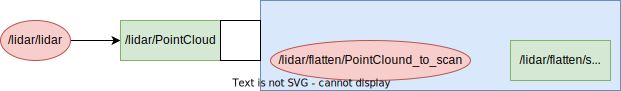
\includegraphics[scale=0.65]{Figures/draw.io/sipleRqtRos1.drawio.pdf}
  \caption{Simplifyed node-graph of ROS1 system}
  \label{fig:simpleRos1Rqt}
\end{figure}

\subsubsection{\textit{launch}}
The system is brought up with the help of launch files. One launch file (two in practice) is used to launch the entire ROS1 system, except the ROS1 bridge. The master launch file(s) are responsible for calling upon other "sublaunch" files. The sublaunch file system allows similar functionality to be re-used, similarly to how functions might be used in c or Python. All of the groups depicted in figure \ref{fig:simpleRos1Rqt} has a sublaunch file associated with it. %\textit{viz.launch} is launched if the argument \textit{viz} is set to \textit{true}.

The sublaunch files takes in arguments, which can be passed over to the elements being launched. The arguments can be passed to the sublaunch file when it is called, but there are default settings that are applied for the arguments not specified when the launch file is run. The arguments are passed down either to the nodes or the launch files that are called upon. Some of the arguments are used so that one launch file can called by different launch files without them interfering with each other, by for example changing the prefix on nodes and topics, like mentioned above. The following sections will go over the different launch files. The launch files can be found in Appendix \ref{Appdix:LaunchFiles}.

\subsubsubsection{\textit{flatten.launch}}\label{subsubsec:flatten.launch}
"\textit{flatten.launch}" is used to launch the \textit{pointcloud\_to\_laserscan\_node} 
node of the \textit{pointcloud\_to\_laserscan} package form \cite{ros2-pointcloud-laserscan}. The \textit{pointcloud\_to\_laserscan\_node} node is used to convert a 3D point cloud to a 2D laser scan \cite{pcl_ros}. The conversion will include objects within a given height range set by two arguments, "\textit{min\_height}" and "\textit{max\_height}". The \textit{pointcloud\_to\_laserscan\_node} node subscribes to the \textit{cloud\_in} topic, and expect a message on the \textit{sensor\_msgs/PointCloud2} message format \cite{pcl_ros}. \textit{remap} is used to make the node more generic by allowing the subscribed topic to be set by an argument. The node publishes on the \textit{scan} topic with the \textit{sensor\_msgs/LaserScan} message format. The node is launched within a group with a name space (NS) which adds a NS prefix to the name of the launched node and the published topic.

\subsubsubsection{\textit{lidar.launch}}\label{subsubsec:lidar.launch}
\textit{lidar.launch} is responsible for launching and configuring the nodes for the lidar. A launch file that are included in the packages for the lidar is used to bring up the lidar system, which  consists of several nodes. Some arguments are passed to the lidar launch file, some notable are the \textit{ouster\_ns} - and the  \textit{timestamp\_mode} arguments. The \textit{ouster\_ns} argument is responsible for the second \textit{/lidar} group within the \textit{/lidar} group as seen in figure \ref{fig:Appdix:rqt:ros1_noBridge}. However, this \textit{/lidar/lidar} are represented by a single node in the simplified node graph in figure \ref{fig:simpleRos1Rqt}. A remapping of the standard point cloud topic name is done to make it configurable, trough an argument, and more fitting with the naming scheme of the rest of the system. \textit{flatten.launch} (\ref{subsubsec:flatten.launch}) is called upon, and the \textit{input\_PointCloud} argument is set to the same topic name as the point cloud from the lidar are published on. \textit{min\_height} and \textit{max\_height} are set to $-1 m$ and $1 m$ respectively. These values seems to work fine, but the \textit{max\_height} could have been reduced some. The lidar package was downloaded from \cite{ouster-ros-driver}

A \textit{static\_transform\_publisher} node fromthe \textit{tf2\_ros} package is used to crate a "dummy"-frame on top of the frame for the lidar provided by the lidar-package. This done so that the name of the frame can be altered trough an argument, making it more generic. A second \textit{static\_transform\_publisher} node is used to relate the lidar's position to the rest of the system. The \textit{parent\_link\_name} argument is used to set the name of the parent link of the lidar, so it can be associated with any frame. The \textit{pos} argument describes the transform between the lidar's frame and the parent frame. See \ref{Appdix:lidar.launch} to see the code for the launch file.

\subsubsubsection{\textit{radar.launch}}\label{subsubsec:radar.launch}
\textit{radar.launch} has a somewhat similar structure to \textit{lidar.launch} \ref{subsubsec:lidar.launch}, but is used for launching the radars and not the lidar. \textit{radar.launch} is a heavily modified version of the launch file intended for the radar-modules, included with the radar package (\textit{awr1843boost\_test.launch}). The original launch file did not allow certain arguments to be altered, thus it was necessary to create a new launch file, instead of calling the original. See \cite{ti-mmwave-rospkg} for the radar package, which was slightly altered for this project. A group with a configurable NS is set for the nodes and topics, similar to the other launch files. A remapping of the standard point cloud topic name is done for similar reasons as in \textit{lidar.launch} \ref{subsubsec:lidar.launch}, but also to allow multiple radar modules to be launched. The \textit{ti\_mmwave\_rospkg} node of the \textit{ti\_mmwave\_rospkg} package is responsible for interfacing with the radar modules, by publishing their data as point clouds on the ROS network. The \textit{command\_port} - and the \textit{data\_port} argument has been altered to \textit{/dev/ttyACM\$(arg command\_port\_number)} and \textit{/dev/ttyACM\$(arg data\_port\_number)}, respectively. These arguments is used to inform the node about the file path of the communication link to the radar module, thus it is critical that these can be changed when more than one radar module is used. The file path arguments are set such that only a integer needs to be passed in to the launch file, the rest of the file path does not change (at least for the systems utilised in this project). The \textit{frame\_id} argument is used to set the name of the frame of which the centre of the radar sits. \textit{frame\_id} is set to be \textit{\$(arg radar\_ns)/atenna\_center}, which is a frame located at the centre of the antenna patch of the radar URDF, which will be explained further below. The rest of the arguments are similar to those in the original launch file. 

The \textit{mmWaveQuickConfig} node of the \textit{ti\_mmwave\_rospkg} package is used to provide the radar module with a configuration file. This seems to be a necessary step for the radar to start operating. Radar configuration files can be created with a web tool, but a pre-made configuration file is used, just as in the original launch file. Two \textit{static\_transform\_publisher} nodes are used for similar purposes as those used in \textit{lidar.launch} \ref{subsubsec:lidar.launch}. The points published by the \textit{ti\_mmwave\_rospkg} node are practically speaking two dimensional. However, the points are published at the \textit{sensor\_msgs/PointCloud2} message format. \textit{flatten.launch} \ref{subsubsec:flatten.launch} is used similarly as in \textit{lidar.launch} \ref{subsubsec:lidar.launch}. The \textit{robot\_state\_publisher} node of the \textit{robot\_state\_publisher} package is used make a description of the radar module available on the ROS network. This description is defined in a URDF file. Some remapping are done to allow multiple descriptions to be initialised at the same time. The parameter \textit{tf\_prefix} is set to avoid name conflicts between the frames of different descriptions. See \ref{Appdix:radar.launch} to see the code for the launch file.

\subsubsubsection{\textit{merge.launch}}\label{subsubsec:merge.launch}
The \textit{merge.launch} launch file is used to launch the \textit{laserscan\_multi\_merger} node of the \textit{ira\_laser\_tools} package from \cite{ira-laser-tools}. This node subscribes to a list of \textit{sensor\_msgs/LaserScan} type topics provided by the \textit{laserscan\_topics} argument, and combines them. The node publishes a point cloud and a laser scan, but the laser scan provided by the node did not behave as expected. However, the point cloud did seem to consist of data similar to the input messages, thus this was used. The merged point cloud gets passed in to \textit{flatten.launch} \ref{subsubsec:flatten.launch}, which produces the final, merged, scan message.

\subsubsubsection{\textit{mount.launch}}\label{subsubsec:mount.launch}
The \textit{mount.launch} launch file is used to make a description of the radar mount available on the ROS network, in a similar manner as in \textit{radar.launch} \ref{subsubsec:radar.launch}. The URDF-file of the mount produces three frames that represent locations where radar modules can be mounted. \textit{static\_transform\_publisher} nodes are used to place frames on top of the existing, where the names of the new frames can be set with arguments. A \textit{static\_transform\_publisher} node is used to create a transform between the base of the mount description and the rest of the system.

\subsubsubsection{\textit{viz.launch}} 
\textit{viz.launch} is used to launch two visualisation tools of ROS, \textit{rqt} and {rviz}. \textit{rqt} appears to open with the same settings as it was closed with, thus no "special" configuration is required. \textit{rviz} on the other hand will (seemingly) automatically open a standard configuration, which forces the user to configure \textit{rviz} each time it is opened. A file containing settings for \textit{rviz} has been created and this file are called when \textit{rviz} gets launched, this solves solves the issue with having to apply settings each time the program is run.

\subsubsubsection{\textit{launchNoRadar1.launch}}\label{subsubsec:launchNoRadar1.launch}
\textit{launchNoRadar1.launch} is one of two launch files that are launched "manually" and not trough a different launch file. These can be viewed as "main" launch files, as they call other launch files, and does not initialise any nodes directly. \textit{viz.launch} is launched if the argument \textit{viz} is set to \textit{true} when \textit{launchNoRadar1.launch} is called. \textit{mount.launch} is launched before the radars to ensure that the mount frames exists when the radars are launched. The mount is rotated about the $x$ axis, of the base frame of the robot, with $\frac{\pi}{2} rad$ trough the \textit{pos} argument. \textit{radar.launch} \label{subsubsec:radar.launch} is called with the argument \textit{radar\_ns} set to \textit{radar0}. The \textit{parent\_link\_name} argument is set to \textit{radar\_pos1}, and the \textit{command\_port\_number} - and \textit{data\_port\_number} arguments are set to \textit{0} and \textit{1}, respectively. The \textit{lidar.launch} \ref{subsubsec:lidar.launch} launch file is called with the \textit{pos} argument set such that the lidar are placed and rotated propperly. The $x$, $y$ and $z$ coordinates of the radar were obtained by summing the transforms and the URDF of the lidar from \cite{uia_husky_0776}. The lidar are mounted backwards, this is corrected by rotating it $\pi rad$ about the $z$ axis. Lastly, the \textit{merge.launch} \ref{subsubsec:merge.launch} launch file is called. The only argument that is passed passed to the \textit{merge.launch} \ref{subsubsec:merge.launch} launch file is the \textit{command\_port\_number} argument, this is configured so it share the base frame with the rest of the ROS1 system.

\subsubsubsection{\textit{launchRadar1.launch}}\label{subsubsec:launchRadar1.launch}
\textit{launchRadar1.launch} and \textit{launchNoRadar1.launch} \ref{subsubsec:launchNoRadar1.launch} where originally part of the same launch file, but they where split up due to some technical issues. The process of launching the radars seem to consist of two steps, configuration and reading data. The issue seems to surround the configuration part. The behaviour of the configuration appears to be unpredictable, and it can take several launching attempts and restarts of the radar modules to successfully launch the radars. The radars have been launched by at a point, but is was a lot less reliable than the current solution. The Github pages associated with the \textit{ti\_mmwave\_rospkg} package seems to suggest that is difficult to launch several radars at the same time due to conflicts with the USB-communication. The second radar is launched by calling \textit{radar.launch} \ref{subsubsec:radar.launch}, but this time with different arguments. The \textit{radar\_ns} argument is set to \textit{radar1}, the \textit{radar.launch} - and the argument is set to \textit{2} and \textit{3}, respectively. 

\subsubsubsection{\textit{lidar.launch}}\label{subsubsec:lidar.launch}
A third "main" launch file was also created to launch only the lidar, called \textit{lidar.launch} see appendix \ref{Appdix:lidar.launch}. This launch file can be used instead of \textit{launchRadar1.launch} and \textit{launchNoRadar1.launch} when testing with just the lidar. The system will behave practically similar, just without the radars.

\subsection{ROS2 system}
The ROS2 system explained with less detail than the ROS1 system, as the main focus has been on the ROS1 system. The ROS2 system do not posses a launch system similar to the ROS1 system. A brief explanation are given for some of the nodes that are used in the ROS2 system, but most of them are re-used from \cite{uia_husky_0776}. 

\subsubsection{\textit{uia\_husky\_0776}}\label{subsubsec:uia_husky_0776}
\textit{uia\_husky\_0776} is not a package, but a collection of packages that are used to operate the Husky. \textit{uia\_husky\_0776} exists as a GitHub repository and it is sheared between three projects, this project, \cite{muggerud2023} and \cite{ovsthus2023}. This repository was created mostly by \cite{ovsthus2023}, as this project required (at some point) the Husky to be operated trough Galactic instead of Foxy, which was used in a earlier version of \cite{uia_husky_0776}. The \textit{husky\_group} package that can be used to launch the Husky, both physically and in simulation, and several launch - and parameter files used in this project are modified version of launch - and parameter files from this package. The \textit{uia\_master\_husky} package is, in short, a modified version of Clearpath's ROS2 Galactic packages for the Huksy, where the modifications where made by \cite{ovsthus2023}. The \textit{um7} package is used to communicate with the IMU, and to make its data available on the ROS2 network. The \textit{serial} package, from \cite{serial-communication-library}, is simply used by the \textit{um7} package for serial communication. The process of installing and running the consists of the \textit{uia\_husky\_0776} repository is explained quite well on its \href{https://github.com/orjano-max/uia_husky_0776}{Github page}.

\subsubsection{\textit{ros1\_bridge}}\label{subsubsec:ros1_bridge}
The \textit{ros1\_bridge} package contains a network bridge that allows messages to be exchanged between ROS1 and ROS2 \cite{ros1_bridge}. The bridge will only carry messages in situations where one side sends a message that gets subscribed to on the other side, at least by default. This done to increase computational efficiency \cite{ros1_bridge}. The bridge can be tested by running the command below in ROS2. 

\begin{tcolorbox}[width=\textwidth,colback={black},colupper=white, title={ubuntu terminal},colbacktitle=gray!125,coltitle=gray!50]\label{shell:echo}    
   \mint{shell}{ros2 topic echo <topic-name> <topic-type>}
\end{tcolorbox}  

Running this command will cause a topic to be subscribed to, and its messages to be displayed in the same terminal as the command was run in. \textit{<topic-name>} should be replaced with the name of the desired topic, and \textit{<topic-type>} with the name of the \href{https://docs.ros.org/en/noetic/api/sensor_msgs/html/msg/}{message type}. It is critical that the \textit{/scan} topic are "translated" by the bridge, thus this is what the described method was used for. The \textit{/scan} topic are associated with the \href{https://docs.ros.org/en/noetic/api/sensor_msgs/html/msg/LaserScan.html}{\textit{sensor\_msgs/LaserScan}} message format. Thus the following command is run:

\begin{tcolorbox}[width=\textwidth,colback={black},colupper=white, title={ubuntu terminal},colbacktitle=gray!125,coltitle=gray!50]\label{shell:echo1}    
   \mint{shell}{ros2 topic echo /scan sensor_msgs/LaserScan}
\end{tcolorbox} 

The \textit{/scan} topic should be visible in both \textit{rqt} and \textit{rviz2}, in ROS2, after running this command (assuming it is visible in ROS1). 

\paragraph{Install and run}
The package can be installed differently depending on the use case. Installing the pre-built packages is convenient in this project, as the messages used are relayed properly with this instalment of the bridge. The \textit{ros1\_bridge} package can be installed by running the following command: 

\begin{tcolorbox}[width=\textwidth,colback={black},colupper=white, title={ubuntu terminal},colbacktitle=gray!125,coltitle=gray!50]\label{shell:echo1}    
   \mint{shell}{sudo apt install ros-<ros2 distro>-ros1-bridge}
\end{tcolorbox} 

Where \textit{<ros2 distro>} should be replaced with the name ROS2 distribution used, this would be \textit{Galactic} in this project. Installing the \textit{ros1\_bridge} for \textit{galactic} can be done by running the following command:

\begin{tcolorbox}[width=\textwidth,colback={black},colupper=white, title={ubuntu terminal},colbacktitle=gray!125,coltitle=gray!50]\label{shell:echo1}    
   \mint{shell}{sudo apt install ros-galactic-ros1-bridge}
\end{tcolorbox} 

The bridge, like other packages, have to be sourced before it can be run, but unlike most packages, the bridge requires both ROS1 and ROS2 to be sourced. The bridge itself is sourced together with ROS2, as the binary packages was installed. The following sequence of command can be used to run the bridge.

\begin{tcolorbox}[width=\textwidth,colback={black},colupper=white, title={ubuntu terminal},colbacktitle=gray!125,coltitle=gray!50]\label{shell:echo1}    
   \mint{shell}{source /opt/ros/noetic/setup.bash}
   \mint{shell}{source /opt/ros/galactic/setup.bash} 
   \mint{shell}{ros2 run ros1_bridge dynamic_bridge}
\end{tcolorbox} 

\subsubsection{\textit{teleop\_twist\_joy}}
The \textit{teleop\_twist\_joy} package allows the Husky to be remote controlled by a game-controller, or a joy-stick. This function was served by a different joy-stick package in \cite{uia_husky_0776}, but this solution stopped working after the Husky's onboard computer was re-flashed. The package comes with a launch file that launches two nodes, one reads the inputs from joy-stick an publishes this to the ROS2 network at the \textit{/joy} topic, the other subscribes to the \textit{/joy} topic and translates button presses to velocity messages.

%\subsubsection{\textit{slam\_toolbox}}
\subsubsection{\textit{nav2\_bringup}}\label{subsubsec:nav2_bringup}
NAV2 are responsible for navigation, as already mentioned. NAV2 is a complicated system that can be configured trough a parameter file. Such a parameter file already existed form \cite{uia_husky_0776}. A copy of this file was made, and some alterations was made. Some changes was made so the odometry produced by the extended Kalman filter (EKF) would be used instead of just the standard wheel odometry.

Alterations was also made to the local footprint. The robot footprint essentially tells NAV2 how big the Husky is, which NAV2 can use to determine where it can navigate while avoiding collision. A sketch of the Husky's perimeter was drawn in Solidworks. This sketch was made to accommodate the mounting system, on both bumpers. The points that represent the start and end of the lines making up the sketch were extracted with this technique \cite{extractingXYZPointData}. The points produced by this method was post processed in Visual Studio before their order was checked. The order of the points matters when defining the footprint. The order was tested and corrected with help of a plotter tool called Geogebra.


%\begin{figure}[H]
%\centering
%\includesvg[scale=0.14]{Figures/ros/ros1graph_noBridge.svg}
%  \caption{rqt node-graph of ROS1 system (see %\ref{Appdix:rqtROS1NB} for a bigger figure)}
%  \label{fig:rqt:ros1_noBridge}
%\end{figure}

\subsection{Bring up the system}
The following sections will explain the method used to bring up the system. The bring up method consists of running several commands in the Ubuntu terminal, and they are often system specific. Factors like file paths and IP addresses must likely be changed both in the commands, but also in some of the files discussed in section \ref{sec:ROSsystem}. These instructions also requires all required packages to be installed and built. The \textit{uia\_husky\_0776} \ref{subsubsec:uia_husky_0776} repository was downloaded and built under the directory \textit{husky\_ws}. This file path: \textit{didrik\_ws/src/Master-thesis-Didrik-Robsrud} is replaced with \textit{<path>} to save space in the following terminal boxes. 

The commands are divided in two, those who runs on the Husky's computer and those run on the operator computer. The order of which the commands are run seem to be arbitrary, but a order was developed to better deal with the unpredictability of hardware/software. The order for the operator computer is arbitrary, and not all of the commands are necessary, depending on what the operator intend to achieve. All of these commands are intended to be executed on the operator computer.

\subsubsection{System bring up}
All the command-sequences in this section starts with connecting to the Husky's onboard computer trough SSH. The first command-sequence are used to bring up the Husky, because an issue with the Husky's USB connection would often arise. This was solved by first turning off the USB-port of the USB-hub, which connected the Husky, IMU, radar modules to the computer, where the Husky was plugged in, then disconnecting and re-connecting the USB-hub from/to the computer, then turning the USB-port back on again. This method was discovered by \cite{ovsthus2023}. This reset will break the connection to the radar modules, thus the Husky is launched first.

\begin{tcolorbox}[width=\textwidth,colback={black},colupper=white, title={ubuntu terminal},colbacktitle=gray!125,coltitle=gray!50]\label{shell:echo1}    
   \mint{shell}{ssh husky@192.168.0.169}
   \mint{shell}{source husky_ws/install/setup.bash} 
   \mint{shell}{ros2 launch <path>/launch1/husky/husky.launch.py}
\end{tcolorbox}

Communication access is granted trough the \textit{chmod} commands, then then the ROS1 system is launched, minus radar1.

\begin{tcolorbox}[width=\textwidth,colback={black},colupper=white, title={ubuntu terminal},colbacktitle=gray!125,coltitle=gray!50]\label{shell:echo1}    
   \mint{shell}{ssh husky@192.168.0.169}
   \mint{shell}{sudo chmod 666 /dev/ttyACM0} 
   \mint{shell}{sudo chmod 666 /dev/ttyACM1}
   \mint{shell}{source didrik_ws/devel/setup.bash}
   \mint{shell}{roslaunch launch launchNoRadar1.launch}
\end{tcolorbox} 

Then radar1 is launched.

\begin{tcolorbox}[width=\textwidth,colback={black},colupper=white, title={ubuntu terminal},colbacktitle=gray!125,coltitle=gray!50]\label{shell:echo1}    
   \mint{shell}{ssh husky@192.168.0.169}
   \mint{shell}{sudo chmod 666 /dev/ttyACM2} 
   \mint{shell}{sudo chmod 666 /dev/ttyACM3}
   \mint{shell}{source didrik_ws/devel/setup.bash}
   \mint{shell}{roslaunch launch launchRadar1.launch}
\end{tcolorbox} 

Both ROS1 and ROS2 are sourced, the the ROS1 bridge is run.

\begin{tcolorbox}[width=\textwidth,colback={black},colupper=white, title={ubuntu terminal},colbacktitle=gray!125,coltitle=gray!50]\label{shell:echo1}    
   \mint{shell}{ssh husky@192.168.0.169}
   \mint{shell}{source /opt/ros/noetic/setup.bash} 
   \mint{shell}{source /opt/ros/galactic/setup.bash}
   \mint{shell}{ros2 run ros1_bridge dynamic_bridge}
\end{tcolorbox} 

NAV2 is launched with its appropriate parameter file.

\begin{tcolorbox}[width=\textwidth,colback={black},colupper=white, title={ubuntu terminal},colbacktitle=gray!125,coltitle=gray!50]\label{shell:echo1}    
   \mint{shell}{ssh husky@192.168.0.169}
   \mint{shell}{source /opt/ros/galactic/setup.bash} 
   \mint{shell}{ros2 launch slam_toolbox lifelong_launch.py use_sim_time:=false}
   \mint{shell}{slam_params_file:=<path>/launch1/husky/params/mapper_params_lifelong.yaml}
\end{tcolorbox} 
\textbf{Where the two last lines should be executed together.}

SLAM toolbox is launched with a parameter file.

\begin{tcolorbox}[width=\textwidth,colback={black},colupper=white, title={ubuntu terminal},colbacktitle=gray!125,coltitle=gray!50]\label{shell:echo1}    
   \mint{shell}{ssh husky@192.168.0.169}
   \mint{shell}{source /opt/ros/galactic/setup.bash} 
   \mint{shell}{ros2 launch nav2_bringup navigation_launch.py}
   \mint{shell}{params_file:=<path>/launch1/husky/params/nav2_params.yaml}
\end{tcolorbox}
\textbf{Where the two last lines should be executed together.}

\subsubsection{Operator bring up}
Launch ROS1 visualisation tools, Rviz and rqt.
\begin{tcolorbox}[width=\textwidth,colback={black},colupper=white, title={ubuntu terminal},colbacktitle=gray!125,coltitle=gray!50]\label{shell:echo1}    
   \mint{shell}{source didrik_ws/devel/setup.bash}
   \mint{shell}{export ROS_MASTER_URI=http://192.168.0.169:11311} 
   \mint{shell}{roslaunch launch viz.launch}
\end{tcolorbox}

Launch ROS2 Rviz2.

\begin{tcolorbox}[width=\textwidth,colback={black},colupper=white, title={ubuntu terminal},colbacktitle=gray!125,coltitle=gray!50]\label{shell:echo1}    
   \mint{shell}{source husky_ws/install/setup.bash}
   \mint{shell}{rviz2 <path>/launch1/rviz/ros2viz.rviz} 
\end{tcolorbox}

Launch ROS2 rqt.

\begin{tcolorbox}[width=\textwidth,colback={black},colupper=white, title={ubuntu terminal},colbacktitle=gray!125,coltitle=gray!50]\label{shell:echo1}    
   \mint{shell}{source /opt/ros/galactic/setup.bash}
   \mint{shell}{rqt} 
\end{tcolorbox}

Launch the joy-stick package.

\begin{tcolorbox}[width=\textwidth,colback={black},colupper=white, title={ubuntu terminal},colbacktitle=gray!125,coltitle=gray!50]\label{shell:echo1}    
   \mint{shell}{source /opt/ros/galactic/setup.bash}
   \mint{shell}{ros2 launch teleop_twist_joy teleop-launch.py joy_config:='xbox'} 
\end{tcolorbox}

%\begin{table}[h!]
%\centering

%\begin{tabular}{c |c| c}
%                &   Laptop              &   SBC and Laptop  \\
%    \hline
%    Ubuntu      &   18.04 (Bionic)      &   20.04 (Focal)   \\
%    \hline
%    ROS1        &   Melodic Morenia     &   Noetic Ninjemys \\  
%    \hline
%    ROS2        &   Eloquent Elusor     &   Galactic Geochelone\\
%\end{tabular}
%\caption{Table to test captions and labels.}
%\label{table:1}
%\end{table}